\documentclass[10pt]{article}
\usepackage[T1]{fontenc}
\usepackage[utf8]{inputenc}
\usepackage{lmodern}
\usepackage[margin=0.7in]{geometry}
\usepackage{amsmath,amssymb}
\usepackage{microtype}
\usepackage{graphicx}
\usepackage{float}
\usepackage[font=small,labelfont=bf,skip=3pt]{caption}
\captionsetup[figure]{font=footnotesize}
\setlength{\parskip}{2pt}
\setlength{\parindent}{0pt}
\setlength{\intextsep}{6pt}
\renewcommand{\thefigure}{\arabic{section}\alph{figure}}
\makeatletter\@addtoreset{figure}{section}\makeatother
\makeatletter
\renewcommand\maketitle{\begin{center}{\large\bfseries\@title\par}\end{center}}
\makeatother

\title{Next step (i): the checkpoint's figures on TinyStories-30M and Shakespeare}

\begin{document}
\maketitle
\vspace{-0.8em}

Each figure of the checkpoint (TinyStories-10M, first) is redone for TinyStories-30M and character-level Shakespeare,
AdamW and Muon only, with the checkpoint's protocol: one initialization, five shared data orders, each optimizer at the
best of five learning rates (TS-30M: AdamW $2\cdot10^{-3}$, Muon 0.01; Shakespeare: AdamW $3\cdot10^{-4}$, Muon 0.04,
picked by the lowest validation loss along training, as the runs overfit). Every step (checkpoints, marked steps,
fork steps) is scaled by the training length: $\times2$ for TS-30M (20{,}000 steps), $\times0.15$ for Shakespeare
(1500 steps).

\section{Figure 1: how the trajectories differ}

\begin{figure}[H]
\centering
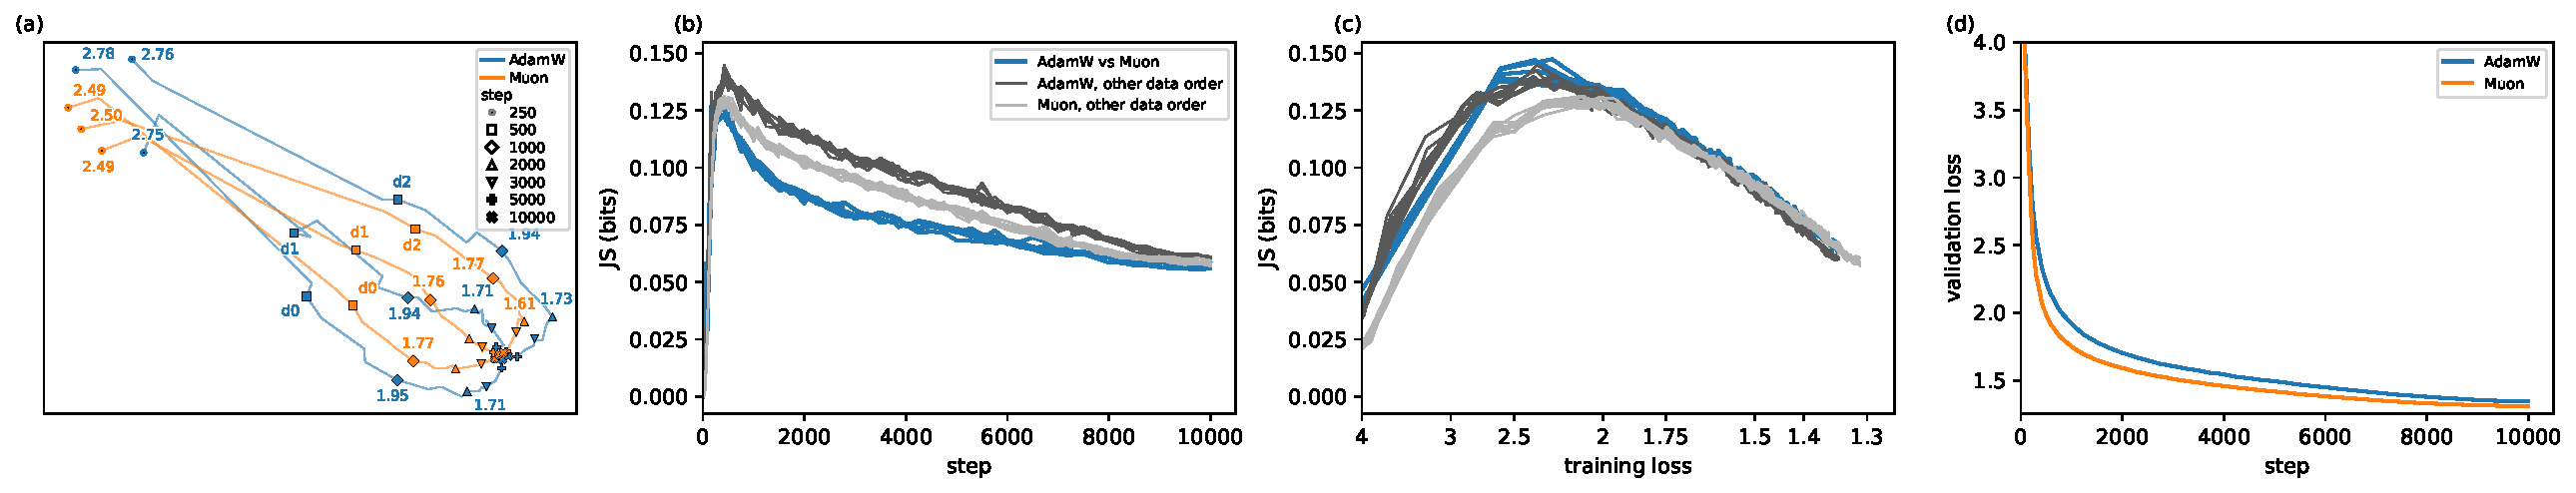
\includegraphics[width=\linewidth]{ts10m/divergence_umap_adamw_muon.pdf}
\caption{TinyStories-10M (the checkpoint's Figure 1). (a) Checkpoints from step 250 on, mapped to 2-D by densMAP;
labels: training loss and data order. (b) JS between runs at equal step. (c) The same at equal training loss. (d)
Validation loss.}
\end{figure}

\begin{figure}[H]
\centering
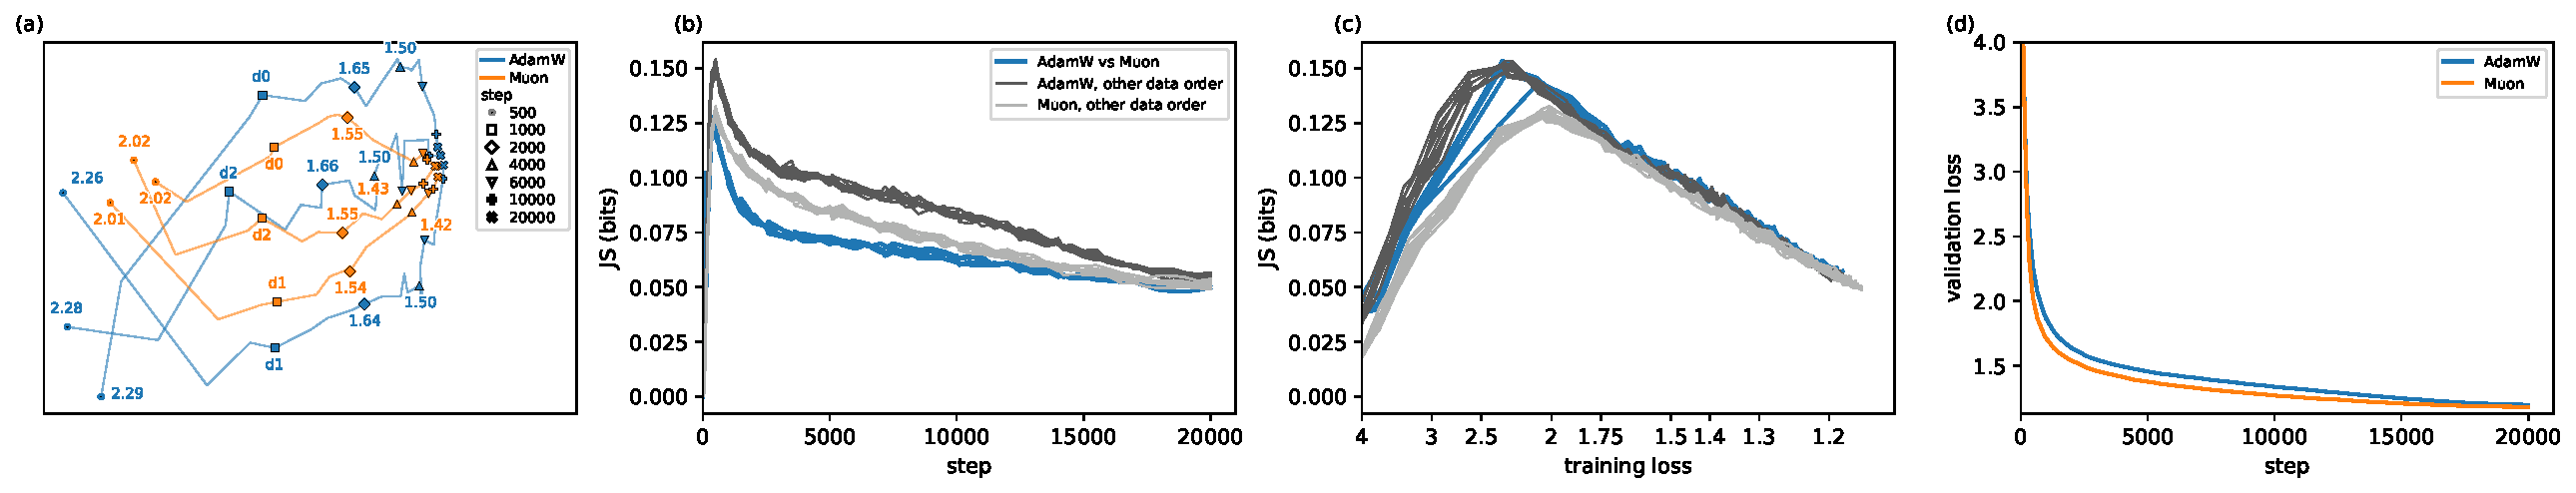
\includegraphics[width=\linewidth]{ts30m/divergence_umap_adamw_muon.pdf}
\caption{TinyStories-30M, as \textbf{1a} with the steps doubled: checkpoints from step 500 on.}
\end{figure}

\begin{figure}[H]
\centering
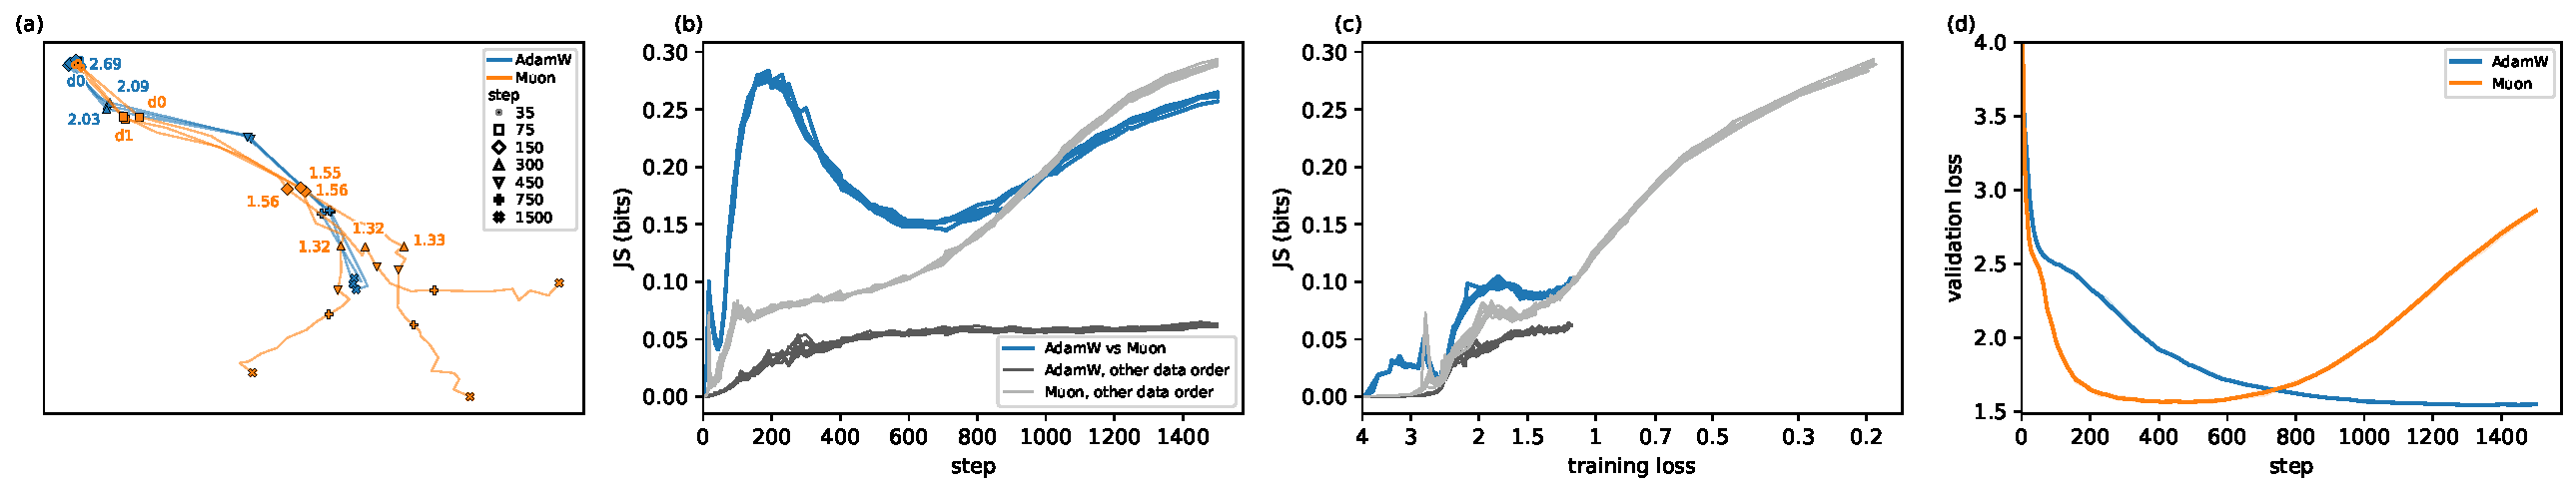
\includegraphics[width=\linewidth]{shakespeare/divergence_umap_adamw_muon.pdf}
\caption{Shakespeare, as \textbf{1a} with the steps $\times0.15$: checkpoints from step 35 on. Muon overfits (d), and
its training loss goes below 1, so (c) uses a log scale in the loss instead of in the loss minus 1.}
\end{figure}

\clearpage
\section{Figure 2: what differs along the way}

\begin{figure}[H]
\centering
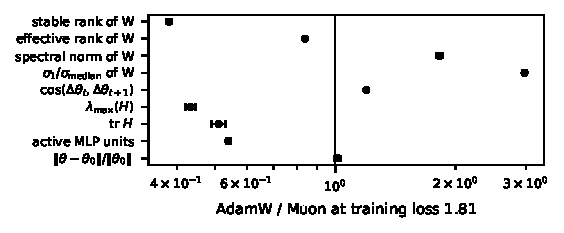
\includegraphics{ts10m/ranking.pdf}
\caption{TinyStories-10M (the checkpoint's Figure 2): ratio AdamW/Muon at training loss 1.81; three data orders each;
bars: range across data orders.}
\end{figure}

\begin{figure}[H]
\centering
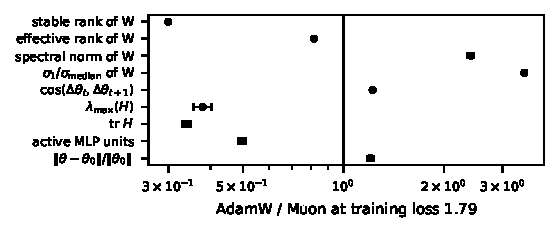
\includegraphics{ts30m/ranking.pdf}
\caption{TinyStories-30M, as \textbf{2a}, at training loss 1.79 (the level of the loss grid nearest 1.81).}
\end{figure}

\begin{figure}[H]
\centering
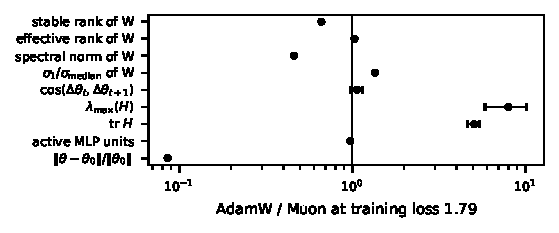
\includegraphics{shakespeare/ranking.pdf}
\caption{Shakespeare, as \textbf{2a}, at training loss 1.79 (the level of the loss grid nearest 1.81).}
\end{figure}

\clearpage
\section{Figure 3: swaps}

\begin{figure}[H]
\centering
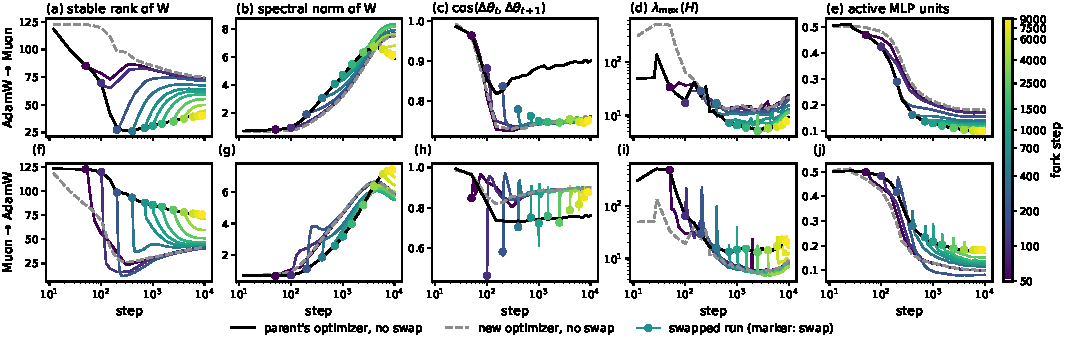
\includegraphics[width=\linewidth]{ts10m/swap_traj_adamw_muon.pdf}
\caption{TinyStories-10M: the checkpoint's Figure 3 with swaps at 6000, 7500 and 9000 added. Top: AdamW to Muon; bottom:
Muon to AdamW. Black: the parent's optimizer without a swap; grey dashed: the new optimizer's own run; colour: swapped
runs, by fork step (dot: the swap).}
\end{figure}

\begin{figure}[H]
\centering
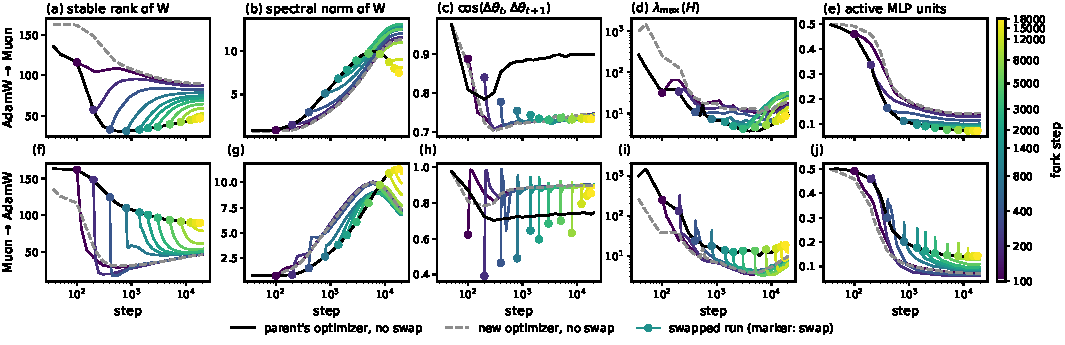
\includegraphics[width=\linewidth]{ts30m/swap_traj_adamw_muon.pdf}
\caption{TinyStories-30M, as \textbf{3a} with the fork steps doubled (100 to 18{,}000).}
\end{figure}

\begin{figure}[H]
\centering
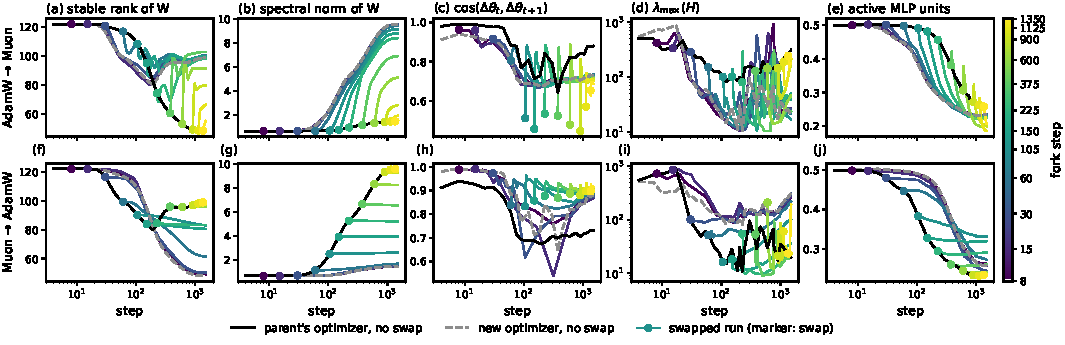
\includegraphics[width=\linewidth]{shakespeare/swap_traj_adamw_muon.pdf}
\caption{Shakespeare, as \textbf{3a} with the fork steps $\times0.15$ (8 to 1350).}
\end{figure}

\end{document}
